%%%%%%%%%%%%%%%%%%%%%%%%%%%%%%%%%%%%%%%%
%
% $ Autor: Gruppe 07 $
% $ Projekt: Magic Faucet Fountain $
% $ Pfad: LaTeXTemplate/Haftungsübernahme/haftungsübernahme.tex $
% $ Kurzbeschreibung: In diesem Dokument wird die Haftungsübernahme der Gruppe behandelt. $
%
% !TeX spellcheck = de_DE/GB
% !TeX program = pdflatex
% !BIB program = biber/bibtex
% !TeX encoding = utf8
%
%%%%%%%%%%%%%%%%%%%%%%%%%%%%%%%%%%%%%%%%


\begin{tikzpicture}
	\node (Logo) at (0mm,0) {
\includegraphics[width=7cm]{Images/Technik}};
	
	
	\node (Adress)  at (10,-22mm) {\begin{tabular}{l} 
			\textbf{\textsf{{\Huge\textcolor{gray}{Der Präsident}}}} \\ 
			\textbf{\textsf{\Large Fachbereich Technik}}\\ 
			\hbox{\vspace{5mm}} \\
			\textbf{\textsf{{\Large\textcolor{gray}{Auskunft erteilt}}}} \\ 
			{\textsf{{Name: Elmar Wings}}}\\ 
			{\textsf{{Name: Elmar.Wings@hs-emden-leer.de}}}\\ 
			{\textsf{{Tel.: 04921 807 1430}}}\\ 
			{\textsf{{Raum: T231}}}\\ 
			
	\end{tabular} };
\end{tikzpicture}	


\vspace{15mm}


\textbf{\textsf{\Large Haftungsübernahme}}

\textsf{System \SystemName}

\vspace{15mm}


\StudentName, \StudentNumber,

\bigskip

übernehmen am \Date{} aus der Hochschule Emden/Leer, Fachbereich Technik, MSR-Labor, folgende Komponenten in einwandfreiem Zustand:

\ListOfMaterials

\StudentName{} haften bis zur Rückgabe persönlich für den Verlust und Schäden, die an den übergebenen Komponenten bis zur Rückgabe entstehen.

\vspace{15mm}

Emden, den \Date


\vspace{15mm}

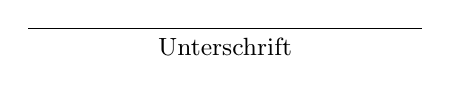
\begin{tikzpicture}
	
	\draw (0,0) -- (50mm,0);
	
	\node[below] (Unterschrift) at (25mm,0) {\small Unterschrift};
	
\end{tikzpicture}	

